\documentclass{beamer}
\usepackage[utf8]{inputenc}
\usepackage[T2A]{fontenc}
\usepackage[russian,english]{babel}
\usepackage{graphicx}
\usepackage{listings}
\usepackage{epstopdf}

\usetheme{Warsaw}

\title{Комбинаторы парсеров}
\subtitle{на примере языка Scala}
\author{Кутепов~А.И.}
\date{2013}

\AtBeginSection[]
{
  \begin{frame}<beamer>
    \tableofcontents[currentsection]
  \end{frame}
}

\begin{document}

\begin{frame}
  \titlepage
\end{frame}

\begin{frame}
  \frametitle{Парсинг}
  \pause
  \begin{block}{Определение}
    \textit{Парсинг} --- процесс сопоставления линейной
    последовательности объектов с некоторым значением или структурой
    данных.
  \end{block}
  \pause
  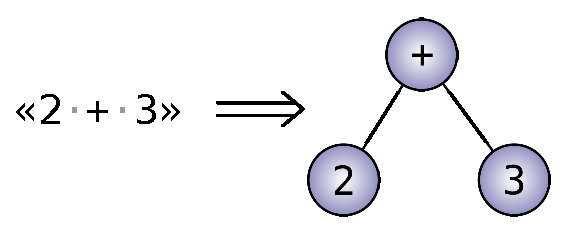
\includegraphics{images/parsing-example.eps}
\end{frame}

\begin{frame}
  \frametitle{Парсер}
  \pause
  \begin{block}{Определение}
    \textit{Парсер} --- функция, которая осуществляет процесс
    \textit{парсинга}.
  \end{block}
  %% FIXME(rexim): not ready yet
  %% \pause
  %% 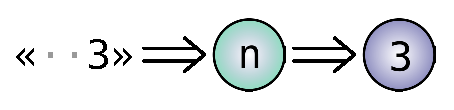
\includegraphics{images/parser-example.eps}
\end{frame}

\begin{frame}
  \frametitle{Комбинатор парсеров}
  \pause
  \begin{block}{Определение}
    \textit{Комбинатор парсеров} --- функция высшего порядка, которая
    в качестве параметров принимает один или более \textit{парсеров} и
    конструирует на их основе новый \textit{парсер}.
  \end{block}
  %% FIXME(rexim): not ready yet.
  %% \pause
  %% \includegraphics{images/paser-combinator-example.ep}
\end{frame}

\end{document}
